\subsection{Flat fielding: calibration stability across the FOV}


The dispersion of the detector responsivity across the field of view has been characterized by estimating flat fields using the \emph{beammap} scans described in Sect.~\ref{se:fp_reconstruction}. We have considered different kinds of flat field:
\begin{itemize}
\item Main beam flat field: the flat field for the far field is estimated using the relative calibration factors obtained for the calibration in FWHM$_{0}$ beam discussed in Sect.~\ref{se:cal_HA}. These are defined as
  \begin{equation}
    G_k = \frac{S_{th}(\nu_0)\, e^{-\tau/sin(\delta)}}{A_k}, 
  \end{equation}
  where $S_{th}(\nu_0)$ is the expected flux of the source integrated in the NIKA2 bandpasses and derived at the reference frequency $\nu_0$, $\tau/sin(\delta)$ is the line-of-sight opacity measured using the \emph{skydip} method described in Sect.~\ref{se:opacities} and $A_k$ is the amplitude of a Gaussian of fixed FWHM fitted from the detector $k$ map (as $A_{c}$ in Eq.~\ref{eq:calib_fix_fwhm}).
\item Forward beam flat field: the flat field for the near field is estimated using the correlation factor of each detector to a median common mode estimated off-source.
\end{itemize}

Figures \ref{fig:avg_mbff} and \ref{fig:avg_fbff} show the average main beam and forward beam flat fields for the three arrays. These have been constructed by combining the normalised flat fields of five \emph{beammap} scans, which were selected using a threshold in the line-of-sight opacity measured in the 1-mm band, such as $\tau/sin(\delta) \leq 0.85$. The dispersion of the average flat fields are shown in the bottom panel of Fig.~\ref{fig:avg_mbff} $\&$ \ref{fig:avg_fbff}. We find a sizable flat field dispersion for Array 1, indicating a significant variation of Array 1 detector responsivities depending on their position in the FOV. This effect, the origin of which is under investigation, mainly impacts the left-most third of the array. We verified that the flat field dispersions for Array 1 are in line with the ones of Array 3 after the detectors of the so-called shadow-zone were flagged out using a crescent-shaped mask. This is evidenced in Fig.~\ref{fig:stddev_ff}, which shows the dispersion of the flat fields for nine \emph{beammap} scans.      


\begin{figure}[ht] 
\begin{center}
  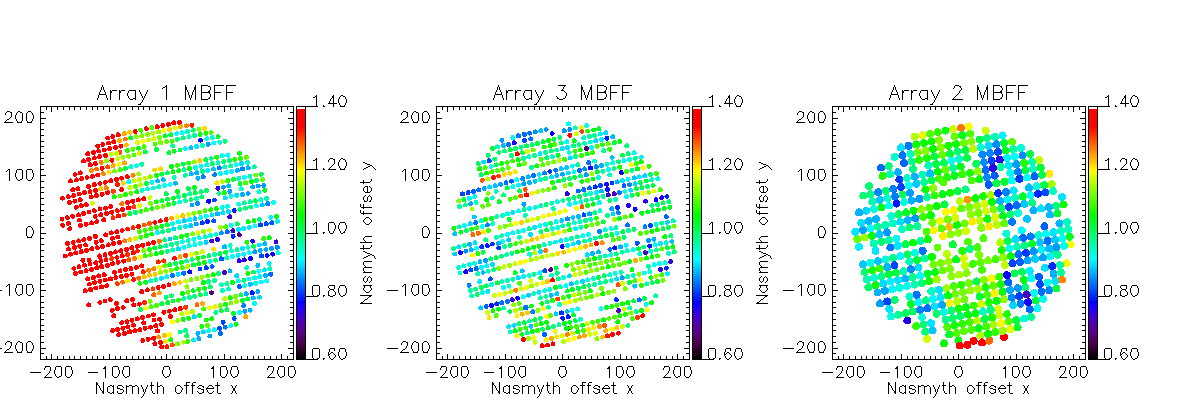
\includegraphics[width=0.95\textwidth]{Figures/FlatFields/Average_main_beam_flat_field_N2R9_10.png}
  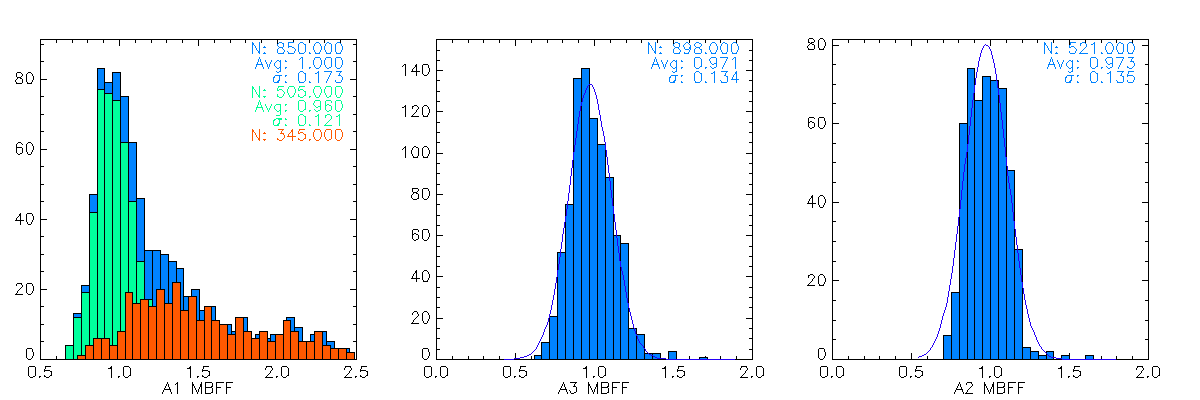
\includegraphics[width=0.8\textwidth]{Figures/FlatFields/Histo_average_main_beam_flat_field_N2R9_10.png}
\caption{Average main beam flat field for array 1, 3 and 2}
 \label{fig:avg_mbff}
\end{center}
\end{figure}

\begin{figure}[ht] 
\begin{center}
  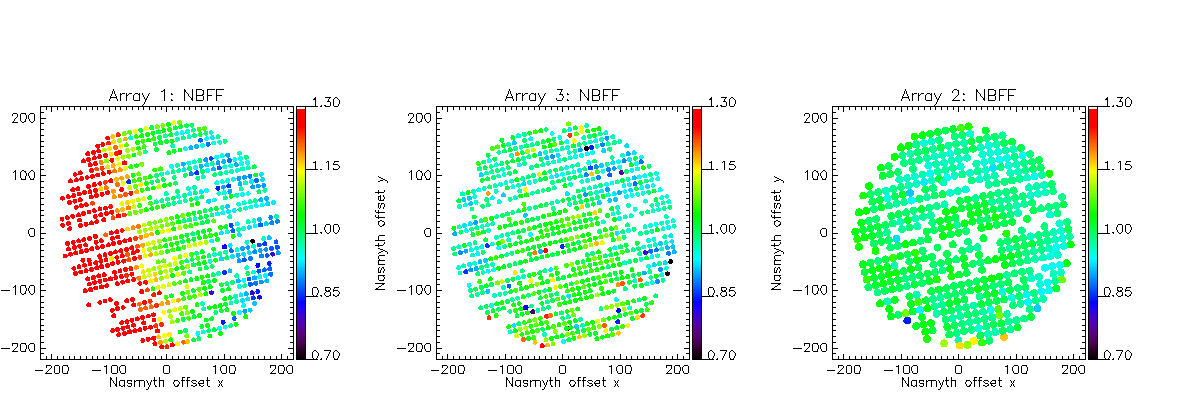
\includegraphics[width=0.95\textwidth]{Figures/FlatFields/Average_near_beam_flat_field_N2R9_10.png}
  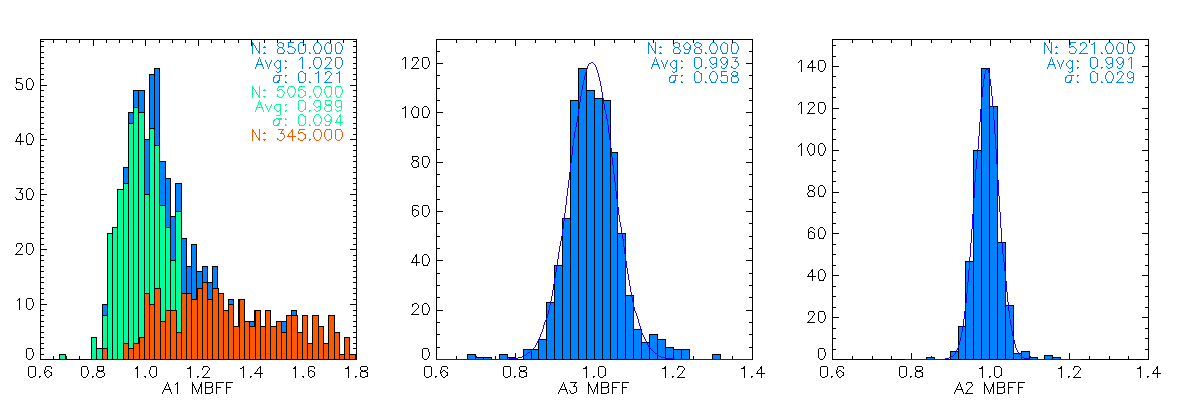
\includegraphics[width=0.8\textwidth]{Figures/FlatFields/Histo_average_near_beam_flat_field_N2R9_10.png}
\caption{Average forward efficiency flat field for array 1, 3 and 2}
 \label{fig:avg_fbff}
\end{center}
\end{figure}

\begin{figure}[ht] 
\begin{center}
  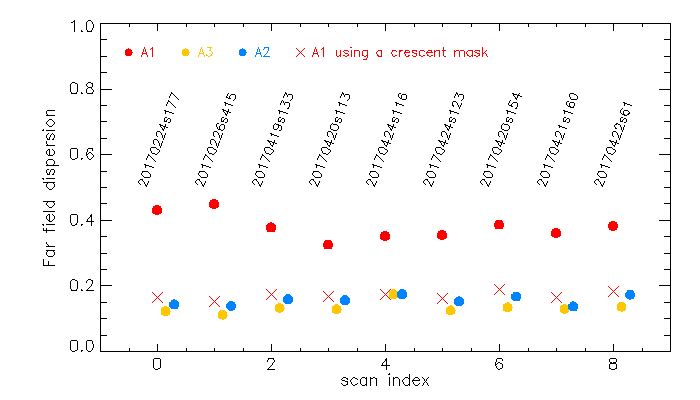
\includegraphics[width=0.6\textwidth]{Figures/FlatFields/Dispersion_main_beam_flat_field_N2R9_10_.png}
  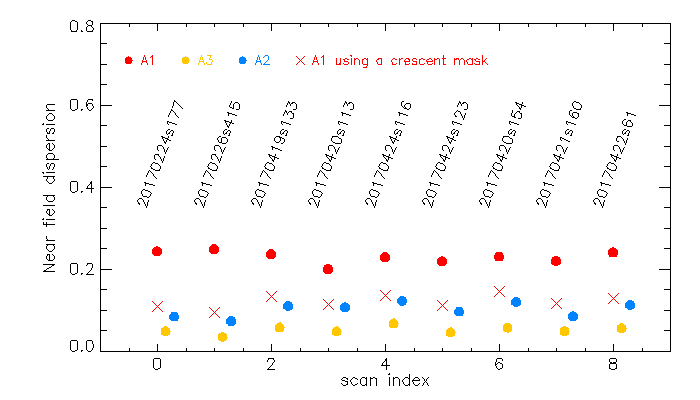
\includegraphics[width=0.6\textwidth]{Figures/FlatFields/Dispersion_forward_beam_flat_field_N2R9_10_.png}
\caption{Dispersion of the flat field for nine \emph{beammap} scans. The RMS dispersion of the main beam flat field (upper panel) and forward beam flat field (lower panel) are shown using all valid KIDs of Array 1 (red circles), Array 3 (orange circles) and Array 2 (blue circles), and using the KIDs located outside the Array 1 "shadow area'', which was discarded using a left crescent-shaped mask (red crosses).}
 \label{fig:stddev_ff}
\end{center}
\end{figure}
